% !TEX root = ../integrado.tex
%=============================================
% Descripción de actores
\label{chapter:ActoresDelSistema}

	En el presente capítulo se definen los participantes en los procesos actuales y fortalecidos. Se da una breve descripción de cada uno, la mayoría tomada de la normatividad correspondiente: Reglamento General, Reglamento interno y Manuales de operación del IPN, entre otros. Aquellas descripciones tomadas de la normatividad tienen la referencia del documento de dónde fueron tomadas, en algunos casos los actores son propuestos para poder llevar a cabo algunas de las tareas en el \refElem{Calmecac}.

\section{Descripción de Actores}

Cada participante se describe con la siguiente estructura:

\begin{objetivos}[Descripción de participantes]
	\item {\bf Nombre:} Nombre con el que se le conoce al participante dentro del negocio.
	\item {\bf Descripción:} Descripción breve del perfil, puesto o rol que juega el participante.
	\item {\bf Área:} En caso de que el participante pertenezca a una estructura se indica el área, departamento o ubicación al que pertenece o se encuentra.
	\item {\bf Responsabilidades:} Se listan las responsabilidades oficiales o relacionadas con el Calmécac según aplique. En el caso de las descripciones tomadas de la normatividad se listan todas.
	\item {\bf Perfil:} Cuando se reconoce un nivel de conocimientos, preparación o capacidades determinadas para desarrollar una participación se describen, con la finalidad de ser tomado en cuenta para el desarrollo del sistema.
	\item {\bf Fuente:} Referencia al documento base de donde fue tomada dicha descripción.
\end{objetivos}

Cuando el participante es un departamento o dirección, se omite el dato ``Perfil'' es un Sistema de Información los datos que se describen son:

\begin{objetivos}[Descripción de sistemas]
	\item {\bf Nombre:} Nombre o siglas del sistema.
	\item {\bf Descripción:} Descripción breve del sistema.
	\item {\bf Área:} Área al que le pertenece, opera o es responsable del sistema.
	\item {\bf Responsabilidades:} Funciones principales del sistema.
	\item {\bf Lenguaje:} Tecnologías principales o plataforma utilizadas en su desarrollo.
	\item {\bf Fuente:} Referencia al documento base de donde fue tomada dicha descripción.
\end{objetivos}

\section{Participantes detectados}

La figura \ref{fig:actoresIN} muestra los actores que participan en el módulo de inscripciones. En particular los actores del submódulo de DAE, DES y UA. %El \refElem{UAResponsableEstructuraEducativa} hereda todas las características de los actores \refElem{UAResponsableHorarios} y \refElem{UAResponsableSD}. 

\begin{figure}[htbp]
	\begin{center}
		\fbox{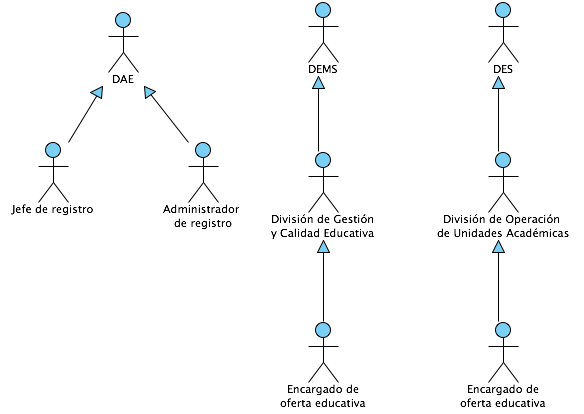
\includegraphics[width=0.7\textwidth]{dinamico/images/Actores_IN}}
		\caption{Actores del módulo de inscripciones}
		\label{fig:actoresIN}
	\end{center}
\end{figure}

%%========== DAEJefeDeRegistro ======%
%\begin{actor}{DAEJefeDeRegistro}{Jefe de Registro}{Persona encarga de registrar los calendarios escolares de las Unidades Académicas y definir el periodo de los procesos de inscripción en el Calmécac.}
%	\item[Área:] \refElem{tDAE}
%	\item[Responsabilidades:] \cdtEmpty
%	\begin{itemize}
%		\item Definir la oferta educativa para los diferentes programas académicos que hay en la unidad académica en sus distintas modalidades para el siguiente periodo escolar.
%		\item Definir la cantidad de grupos a utilizar para la oferta educativa de la unidad académica para el siguiente periodo escolar.
%		\item Asignar unidades de aprendizaje a los grupos que se utilizaran para le siguiente periodo escolar.
%		\item Definir los horarios de las unidades de aprendizaje asignadas a los grupos.
%		\item Definir más de un laboratorio a las unidades de aprendizaje que lo requieran.
%		\item Asignar profesores a las unidades de aprendizaje que se ofertarán para el próximo periodo escolar.
%		\item Asignar a todos los profesores basificados su carga máxima de horas frente a grupo.
%		\item Asignar a los profesores interinos las unidades de aprendizaje 
%		\item Definir un periodo para la recepción de las solicitudes de aprendizaje que son enviadas por los profesores.
%	\end{itemize}
%		\item[Fuente:]%Reglamento General de Estudios, Manual de Organización de la Secretaría Académica
%		%\item[Solicitado por:] 
%\end{actor}
%
%
%========== Responsable de Horarios en la UA ======%
%\begin{actor}{DAEAdministradorDeRegistro}{Administrador de Registro}{Persona encarga de registrar los calendarios escolares de las Unidades Académicas, definir el periodo de los procesos de inscripción en el Calmécac y asignar permisos a usuarios del área.}
%	\item[Área:] \refElem{tDAE}
%	\item[Responsabilidades:] \cdtEmpty
%	\begin{itemize}
%		\item Monitorear las solicitudes de unidades de aprendizaje de los profesores
%		\item Enviar una notificación a los profesores que no halla enviado aún su solicitud de unidades de aprendizaje antes de que se acabe el periodo para la recepción de solicitudes.
%		\item Consultar las solicitudes de los profesores para las diferentes academias que existen en la unidad académica.
%	\end{itemize}
%		\item[Fuente:]%Reglamento General de Estudios, Manual de Organización de la Secretaría Académica
%		%\item[Solicitado por:] 
%\end{actor}
%
%
%%========== DESAdministrador ======%
%\begin{actor}{DESEncargadoDeOfertaEducativa}{Encargado de Oferta Educativa}{Persona encargada de dar seguimiento al proceso de inscripción en la DES.}
%	\item[Área:] \refElem{tDES}
%	\item[Responsabilidades:] \cdtEmpty
%		\begin{itemize}
%			\item Proporcionar información sobre las carreras y lugares ofertados.
%			\item Dar seguimiento al proceso de inscripciones y cambios de carrera.
%		\end{itemize}
%	\item[Fuente:]
%\end{actor}
%
%%========== UAJefeDeControlEscolar ======%
\begin{actor}{UAJefeDeGestionEscolar}{Jefe de Gestión Escolar}{Persona encargada de operar el departamento de Control Escolar de una Unidad Académica.}
	\item[Área:] \refElem{tUA}
	\item[Responsabilidades:] \cdtEmpty
		\begin{itemize}
			\item Operar el CALMÉCAC dentro de la Unidad Académica.
			\item Operar y dirigir el proceso de Reinscripciones junto con el personal de Control Escolar de la Unidad Académica.
		\end{itemize}
	\item[Fuente:]
\end{actor}
